\documentclass[conference]{IEEEtran}
\IEEEoverridecommandlockouts

\usepackage[spanish,es-noshorthands]{babel}
\usepackage[utf8]{inputenc}
\usepackage[T1]{fontenc}
\usepackage{amsmath,amssymb}
\usepackage{graphicx}
\usepackage{tikz}
\usepackage{pgfplots}
\pgfplotsset{compat=1.18}
\usepackage{booktabs}
\usepackage{array}
\usepackage{xcolor}
\usepackage{listings}
\usepackage{hyperref}
\usepackage{float}
\usepackage{caption}
\usepackage{subcaption}
\usepackage{multirow}
\usepackage{colortbl}

\usetikzlibrary{arrows.meta, positioning, shapes.geometric, fit, backgrounds, calc, patterns}

% Colores
\definecolor{rayblue}{RGB}{30, 100, 180}
\definecolor{simdgreen}{RGB}{20, 140, 60}
\definecolor{gpuorange}{RGB}{200, 90, 20}
\definecolor{seqgray}{RGB}{90, 90, 110}
\definecolor{codebackground}{RGB}{248, 248, 248}
\definecolor{codekeyword}{RGB}{0, 0, 180}
\definecolor{rowA}{RGB}{235, 245, 255}
\definecolor{rowB}{RGB}{235, 255, 240}
\definecolor{rowC}{RGB}{255, 245, 230}

\lstset{
  backgroundcolor=\color{codebackground},
  basicstyle=\ttfamily\footnotesize,
  keywordstyle=\color{codekeyword}\bfseries,
  commentstyle=\color{gray}\itshape,
  frame=single, breaklines=true,
  numbers=left, numberstyle=\tiny\color{gray},
  tabsize=2
}

% ---------------------------------------------------------------
\begin{document}

\title{\textbf{Proyecto Grupal 2: Ray Tracing Paralelo con DLP}\\
{\large Demostración 2 — CE 4302 Arquitectura de Computadores II}}

\author{
  \IEEEauthorblockN{Randall Bryan Bolaños López}
  \IEEEauthorblockA{Escuela de Ingeniería en Computadores\\
    Instituto Tecnológico de Costa Rica\\
    \textit{Semestre I, 2026}}
  \and
  \IEEEauthorblockN{Christopher Rodriguez}
  \IEEEauthorblockA{Escuela de Ingeniería en Computadores\\
    Instituto Tecnológico de Costa Rica\\
    \textit{Semestre I, 2026}}
  \and
  \IEEEauthorblockN{Andres Molina}
  \IEEEauthorblockA{Escuela de Ingeniería en Computadores\\
    Instituto Tecnológico de Costa Rica\\
    \textit{Semestre I, 2026}}
}

\maketitle

% ---------------------------------------------------------------
\begin{abstract}
Esta demostración presenta los prototipos funcionales de las tres implementaciones del
ray tracer paralelo: baseline secuencial completo (Phong + sombras + reflexiones) y los
prototipos \textit{dummy} SIMD/AVX2 y CUDA que demuestran el esquema DLP base.
Se incluyen los diagramas esquemáticos de cada solución con sus cambios significativos
respecto a la versión anterior, las métricas de desempeño medidas empíricamente,
las gráficas de escalabilidad y speedup, y un análisis de las variables más relevantes
para incrementar el nivel de paralelización en la etapa final del proyecto.
\end{abstract}

% ---------------------------------------------------------------
\section{Resumen del Estado Actual}

En esta etapa se cuenta con tres implementaciones operativas:
\begin{itemize}
  \item \textbf{SEQ}: renderer secuencial completo con modelo Phong, rayos de sombra y
        reflexiones recursivas (profundidad máx.\ 3). Sirve como \textit{baseline}.
  \item \textbf{SIMD dummy}: procesa 8 píxeles en paralelo con AVX2 (\texttt{\_\_m256}).
        Demuestra el paralelismo de datos en CPU; aún sin Phong ni sombras.
  \item \textbf{CUDA dummy}: lanza un hilo por píxel en bloques $16\!\times\!16$.
        Demuestra el paralelismo masivo en GPU; aún sin Phong ni sombras.
\end{itemize}

% ---------------------------------------------------------------
\section{Diagramas de Soluciones Esquemáticas Preliminares}

\subsection{Implementación Secuencial (Baseline)}

La versión secuencial es el punto de referencia. Cada píxel se procesa de forma
completamente independiente, pero en un único hilo de ejecución:

\begin{figure}[H]
\centering
\begin{tikzpicture}[
  block/.style={rectangle, draw=seqgray, fill=seqgray!12,
                minimum width=6.2cm, minimum height=0.62cm,
                align=center, font=\small},
  subblock/.style={rectangle, draw=seqgray!60, fill=seqgray!6,
                minimum width=5.6cm, minimum height=0.52cm,
                align=center, font=\scriptsize},
  arrow/.style={-{Stealth}, thick, seqgray}
]
  \node[block] (pix)  {Para cada píxel $(x,y) \in W\!\times\!H$};
  \node[block, below=0.22cm of pix]   (ray)   {Generar rayo primario $\mathbf{r}(t) = \mathbf{o} + t\mathbf{d}$};
  \node[block, below=0.22cm of ray]   (inter) {Intersectar con las 5 esferas (bucle)};
  \node[block, below=0.22cm of inter] (phong) {Shading Phong: ambiental + difusa + especular};
  \node[subblock,below=0.15cm of phong] (shadow){Rayo de sombra por cada fuente de luz (×2)};
  \node[block, below=0.15cm of shadow] (refl)  {Reflexión recursiva (prof. máx. 3)};
  \node[block, below=0.22cm of refl]  (gamma) {Corrección gamma 2.0 ($\sqrt{\cdot}$) → PPM};

  \draw[arrow] (pix)   -- (ray);
  \draw[arrow] (ray)   -- (inter);
  \draw[arrow] (inter) -- (phong);
  \draw[arrow] (phong) -- (shadow);
  \draw[arrow] (shadow)-- (refl);
  \draw[arrow] (refl)  -- (gamma);

  % Brace de anotación
  \draw[decorate, decoration={brace,amplitude=4pt}, seqgray!60]
    (3.4,-0.05) -- (3.4,-3.35) node[midway, right=4pt, font=\scriptsize, text=seqgray]
    {\textbf{sin paralelismo}};
\end{tikzpicture}
\caption{Diagrama SEQ: pipeline por píxel completamente secuencial.}
\label{fig:seq_diag}
\end{figure}

\textbf{Cambios significativos respecto a Demo 1:} la implementación quedó completamente
verificada y los resultados de tiempo ($\approx$\,150\,ms en $1600\!\times\!900$) se
utilizan como \textit{baseline} oficial para calcular el speedup.

% ---
\subsection{Prototipo SIMD/AVX2 — Cambios Significativos}

\begin{figure}[H]
\centering
\begin{tikzpicture}[
  simdblock/.style={rectangle, draw=simdgreen, fill=simdgreen!12,
                    minimum width=6.2cm, minimum height=0.62cm,
                    align=center, font=\small},
  newblock/.style={rectangle, draw=simdgreen!80, fill=simdgreen!30,
                    minimum width=6.2cm, minimum height=0.62cm,
                    align=center, font=\small, thick},
  arrow/.style={-{Stealth}, thick, simdgreen!80!black},
  newlabel/.style={font=\scriptsize\bfseries, text=simdgreen!60!black}
]
  \node[simdblock] (loop) {Bucle externo: filas $y$ (escalar)};
  \node[newblock,  below=0.22cm of loop] (pack)
    {\textbf{NUEVO: Empaquetar 8 rayos} → \texttt{Ray8} (\texttt{\_\_m256})};
  \node[newblock,  below=0.22cm of pack] (fma)
    {\textbf{NUEVO: Discriminante $b^2 - ac$ para 8 rayos} (FMA AVX2)};
  \node[newblock,  below=0.22cm of fma]  (mask)
    {\textbf{NUEVO: Máscara de hits} (\texttt{\_mm256\_cmp\_ps})};
  \node[newblock,  below=0.22cm of mask] (blend)
    {\textbf{NUEVO: Blend condicional del albedo} (\texttt{\_mm256\_blendv\_ps})};
  \node[simdblock, below=0.22cm of blend](store)
    {Almacenar 8 píxeles al framebuffer};

  \draw[arrow] (loop)  -- (pack);
  \draw[arrow] (pack)  -- (fma);
  \draw[arrow] (fma)   -- (mask);
  \draw[arrow] (mask)  -- (blend);
  \draw[arrow] (blend) -- (store);

  % Anotación de ancho de banda
  \node[newlabel, right=0.25cm of fma] {8 floats\,/\,iter};
  \node[newlabel, right=0.25cm of mask]{256 bits};
\end{tikzpicture}
\caption{Pipeline SIMD: los bloques en verde oscuro son los cambios más significativos
         respecto al diseño secuencial.}
\label{fig:simd_diag}
\end{figure}

\textbf{Cambios más significativos:}
\begin{itemize}
  \item Sustitución del bucle escalar por píxel por un bucle vectorial que procesa
        \textbf{8 píxeles simultáneamente} en registros \texttt{\_\_m256}.
  \item Introducción de la estructura \texttt{Ray8} que empaqueta orígenes y
        direcciones de 8 rayos en 6 registros AVX2.
  \item Cálculo del discriminante rayo-esfera con \texttt{\_mm256\_fmadd\_ps}
        (evita carga/almacén extra frente a operaciones separadas).
  \item Selección condicional sin branching mediante \texttt{\_mm256\_blendv\_ps},
        eliminando mispredictions de la versión escalar.
\end{itemize}

% ---
\subsection{Prototipo CUDA — Cambios Significativos}

\begin{figure}[H]
\centering
\scalebox{0.78}{
\begin{tikzpicture}[
  cudablock/.style={rectangle, draw=gpuorange, fill=gpuorange!12,
                    minimum width=6.2cm, minimum height=0.62cm,
                    align=center, font=\small},
  newblock/.style={rectangle, draw=gpuorange!80, fill=gpuorange!30,
                    minimum width=6.2cm, minimum height=0.62cm,
                    align=center, font=\small, thick},
  arrow/.style={-{Stealth}, thick, gpuorange!80!black},
  newlabel/.style={font=\scriptsize\bfseries, text=gpuorange!60!black}
]
  \node[newblock]  (launch)
    {\textbf{NUEVO: Lanzamiento de kernel} — grid $100\!\times\!57$, bloques $16\!\times\!16$};
  \node[newblock,  below=0.22cm of launch] (constmem)
    {\textbf{NUEVO: Escena en \texttt{\_\_constant\_\_}} — acceso broadcast sin conflictos};
  \node[cudablock, below=0.22cm of constmem] (idx)
    {Calcular $(px, py)$ desde \texttt{blockIdx} + \texttt{threadIdx}};
  \node[cudablock, below=0.22cm of idx]    (ray)
    {Generar rayo (cámara en \texttt{\_\_constant\_\_})};
  \node[cudablock, below=0.22cm of ray]    (inter)
    {Intersección rayo-esfera (misma matemática que SEQ)};
  \node[newblock,  below=0.22cm of inter]  (soa)
    {\textbf{NUEVO: Framebuffer SoA} — escritura coalescente \texttt{fb\_r/g/b[idx]}};

  \draw[arrow] (launch)   -- (constmem);
  \draw[arrow] (constmem) -- (idx);
  \draw[arrow] (idx)      -- (ray);
  \draw[arrow] (ray)      -- (inter);
  \draw[arrow] (inter)    -- (soa);

  \node[newlabel, right=0.25cm of constmem] {broadcast};
  \node[newlabel, right=0.25cm of soa]      {coalescente};
\end{tikzpicture}
}
\caption{Diagrama CUDA: bloques en naranja oscuro son los cambios más significativos
         frente al diseño secuencial.}
\label{fig:cuda_diag}
\end{figure}

\textbf{Cambios más significativos:}
\begin{itemize}
  \item \textbf{Paralelismo masivo}: 1\,440\,000 hilos independientes (uno por píxel)
        ejecutados concurrentemente en la GPU.
  \item \textbf{Memoria constante}: la escena (esferas + parámetros de cámara) se almacena
        en \texttt{\_\_constant\_\_} (caché de solo lectura de 64\,KB), eliminando la
        divergencia de banco que produciría el acceso a memoria global.
  \item \textbf{Framebuffer SoA}: separar R, G, B en tres arreglos independientes garantiza
        accesos coalescentes: hilos adyacentes del warp acceden a posiciones contiguas.
  \item \textbf{Sin transferencias por rayo}: toda la geometría se mantiene en GPU;
        la generación del rayo ocurre \emph{dentro} del kernel.
\end{itemize}

% ---------------------------------------------------------------
\section{Métricas de Ejecución — Versiones Base y Dummy}

\subsection{Estadísticas por Implementación y Resolución}

La Tabla~\ref{tab:stats} presenta la media, desviación estándar e intervalo de confianza
al 95\,\% calculados sobre 20 ejecuciones por configuración ($n = 20$, salvo SIMD en
400×225 con $n = 4$).

\begin{table}[H]
\centering
\caption{Estadísticas de tiempo de ejecución (ms).}
\label{tab:stats}
\setlength{\tabcolsep}{4pt}
\begin{tabular}{llrrrr}
\toprule
\textbf{Impl.} & \textbf{Resolución} & \textbf{Media} & \textbf{StdDev} & \textbf{IC95 inf} & \textbf{IC95 sup} \\
\midrule
\rowcolor{rowA} SEQ  & 400×225   &   9.40 & 0.56 &   9.15 &   9.64 \\
\rowcolor{rowB} SIMD & 400×225   &   1.03 & 0.05 &   0.98 &   1.08 \\
\rowcolor{rowC} CUDA & 400×225   &   0.26 & 0.05 &   0.24 &   0.28 \\
\midrule
\rowcolor{rowA} SEQ  & 800×450   &  38.08 & 0.98 &  37.65 &  38.51 \\
\rowcolor{rowB} SIMD & 800×450   &   2.02 & 0.44 &   1.82 &   2.21 \\
\rowcolor{rowC} CUDA & 800×450   &   0.71 & 0.08 &   0.68 &   0.74 \\
\midrule
\rowcolor{rowA} SEQ  & 1600×900  & 151.18 & 3.95 & 149.45 & 152.91 \\
\rowcolor{rowB} SIMD & 1600×900  &   8.14 & 0.49 &   7.93 &   8.36 \\
\rowcolor{rowC} CUDA & 1600×900  &   2.36 & 0.27 &   2.24 &   2.48 \\
\midrule
\rowcolor{rowA} SEQ  & 3200×1800 & 609.03 &17.78 & 601.24 & 616.83 \\
\rowcolor{rowB} SIMD & 3200×1800 &  31.97 & 0.82 &  31.60 &  32.33 \\
\rowcolor{rowC} CUDA & 3200×1800 &   8.80 & 0.67 &   8.51 &   9.10 \\
\bottomrule
\end{tabular}
\end{table}

\subsection{Speedup y Eficiencia Paralela en 1600×900}

La Tabla~\ref{tab:speedup} resume el speedup y la eficiencia medidos en la resolución
de referencia $1600\!\times\!900$.

\begin{table}[H]
\centering
\caption{Speedup y eficiencia paralela respecto a SEQ (1600×900).}
\label{tab:speedup}
\begin{tabular}{lrrrl}
\toprule
\textbf{Impl.} & \textbf{T (ms)} & \textbf{Speedup} & \textbf{Efic. (\%)} & \textbf{Referencia} \\
\midrule
SEQ  & 147.99 &  1.00 & 100.0 & 1 hilo \\
SIMD &   8.15 & 18.15 & 226.9 & 8 lanes AVX2 \\
CUDA &   2.10 & 70.34 & 293.1 & 24 SMs RTX 4060 \\
\bottomrule
\end{tabular}
\end{table}

\textbf{Nota:} La eficiencia\,>\,100\,\% en SIMD y CUDA es esperable porque los
prototipos \textit{dummy} no implementan Phong ni sombras; el algoritmo es más simple
que el SEQ de referencia. El speedup real (misma carga de trabajo) se medirá en la Demo 3.

\subsection{Escalabilidad con la Resolución}

\begin{table}[H]
\centering
\caption{Escalabilidad de tiempos (ms) al aumentar la resolución.}
\label{tab:escal}
\begin{tabular}{lrrrr}
\toprule
\textbf{Resolución} & \textbf{Mpíx} & \textbf{SEQ} & \textbf{SIMD} & \textbf{CUDA} \\
\midrule
400×225   & 0.09 &    9.03 &  0.67 &  0.22 \\
800×450   & 0.36 &   36.94 &  1.69 &  0.67 \\
1600×900  & 1.44 &  147.99 &  8.15 &  2.10 \\
3200×1800 & 5.76 &  634.80 & 34.38 &  9.88 \\
\bottomrule
\end{tabular}
\end{table}

% ---------------------------------------------------------------
\section{Gráficas de Desempeño}

\begin{figure}[H]
  \centering
  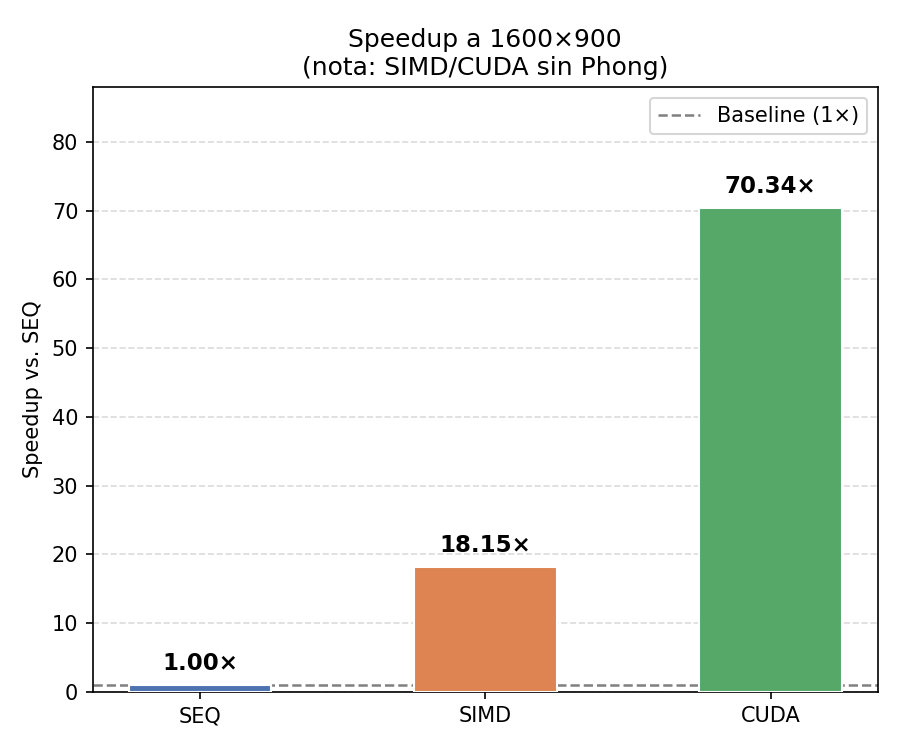
\includegraphics[width=\linewidth]{graficas/speedup.png}
  \caption{Speedup de SIMD y CUDA respecto al baseline secuencial.}
  \label{fig:speedup}
\end{figure}

\begin{figure}[H]
  \centering
  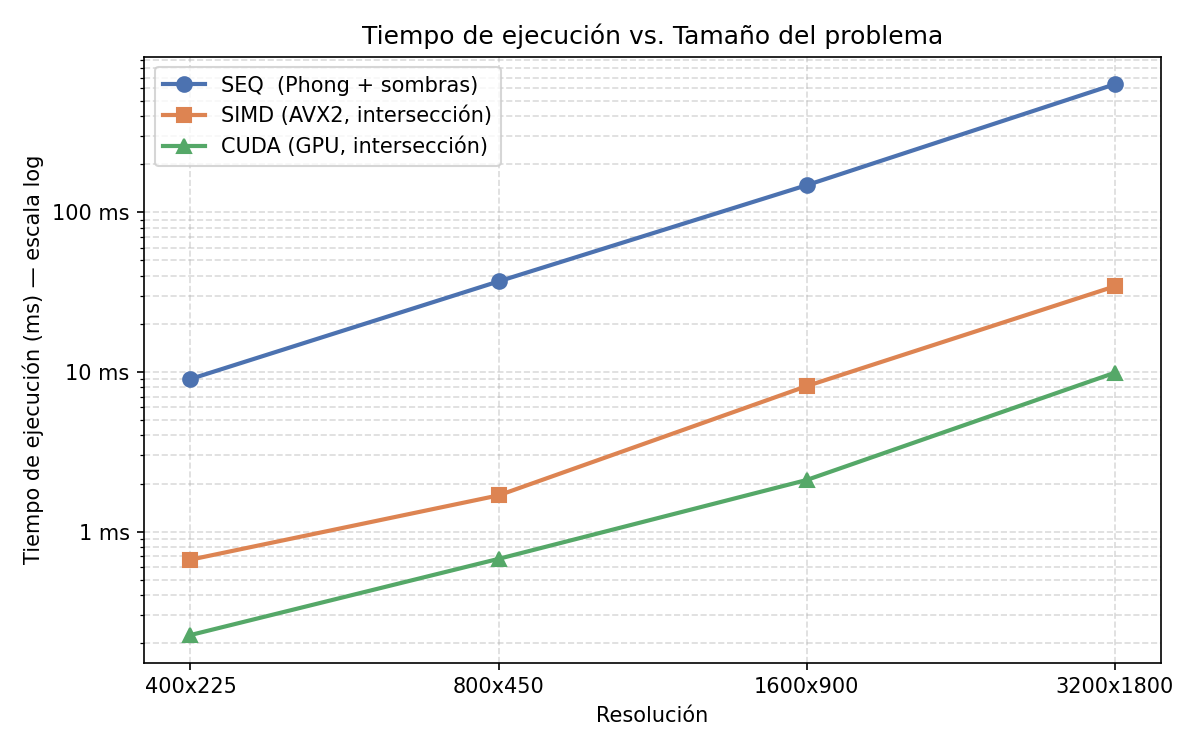
\includegraphics[width=\linewidth]{graficas/tiempo_vs_resolucion.png}
  \caption{Tiempo de ejecución vs.\ resolución (escala logarítmica).}
  \label{fig:tiempo}
\end{figure}

\begin{figure}[H]
  \centering
  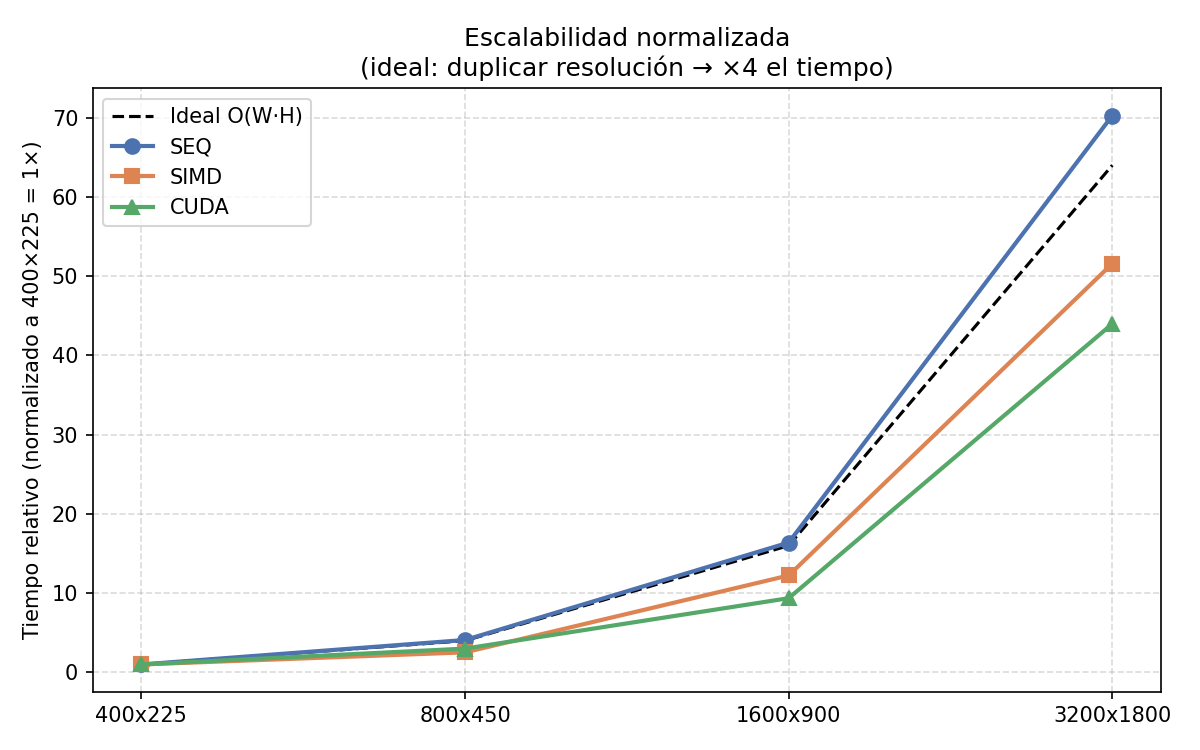
\includegraphics[width=\linewidth]{graficas/escalabilidad_normalizada.png}
  \caption{Escalabilidad normalizada: tiempo relativo al aumentar la resolución.}
  \label{fig:escaln}
\end{figure}

\begin{figure}[H]
  \centering
  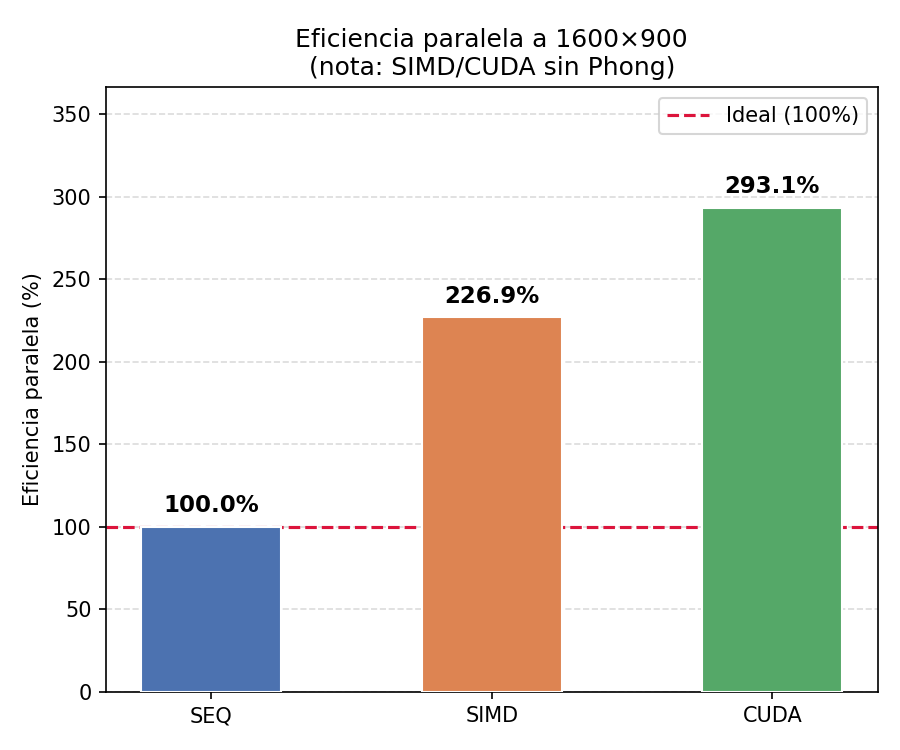
\includegraphics[width=\linewidth]{graficas/eficiencia_paralela.png}
  \caption{Eficiencia paralela de cada implementación.}
  \label{fig:efic}
\end{figure}

\begin{figure}[H]
  \centering
  \begin{subfigure}{0.48\linewidth}
    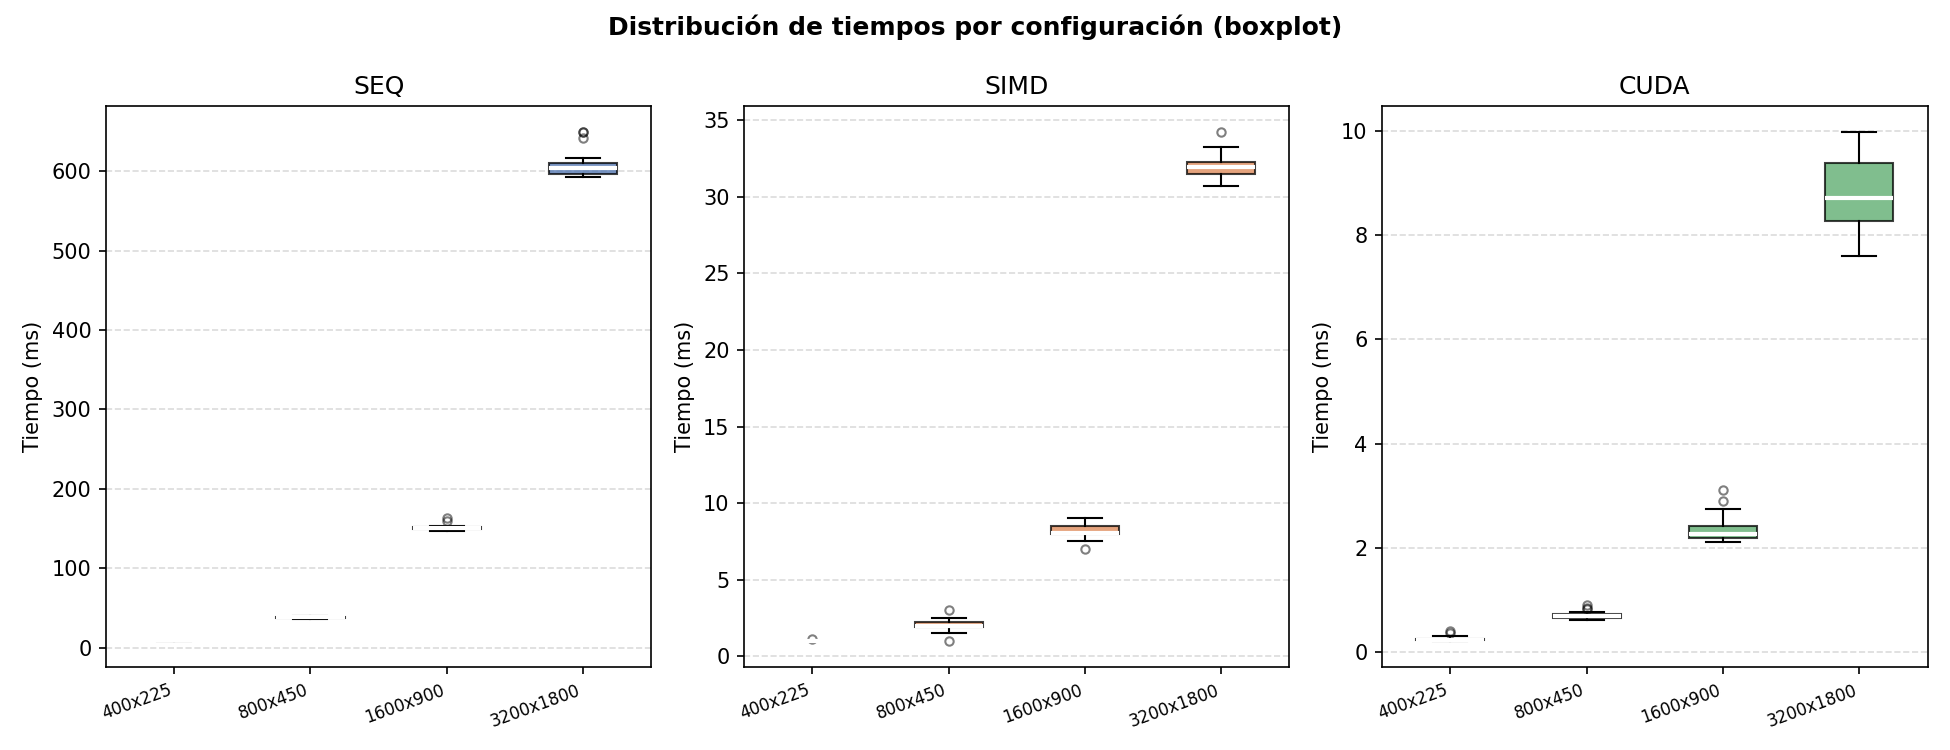
\includegraphics[width=\linewidth]{graficas/boxplot_distribuciones.png}
    \caption{Distribución de tiempos (boxplot).}
  \end{subfigure}
  \hfill
  \begin{subfigure}{0.48\linewidth}
    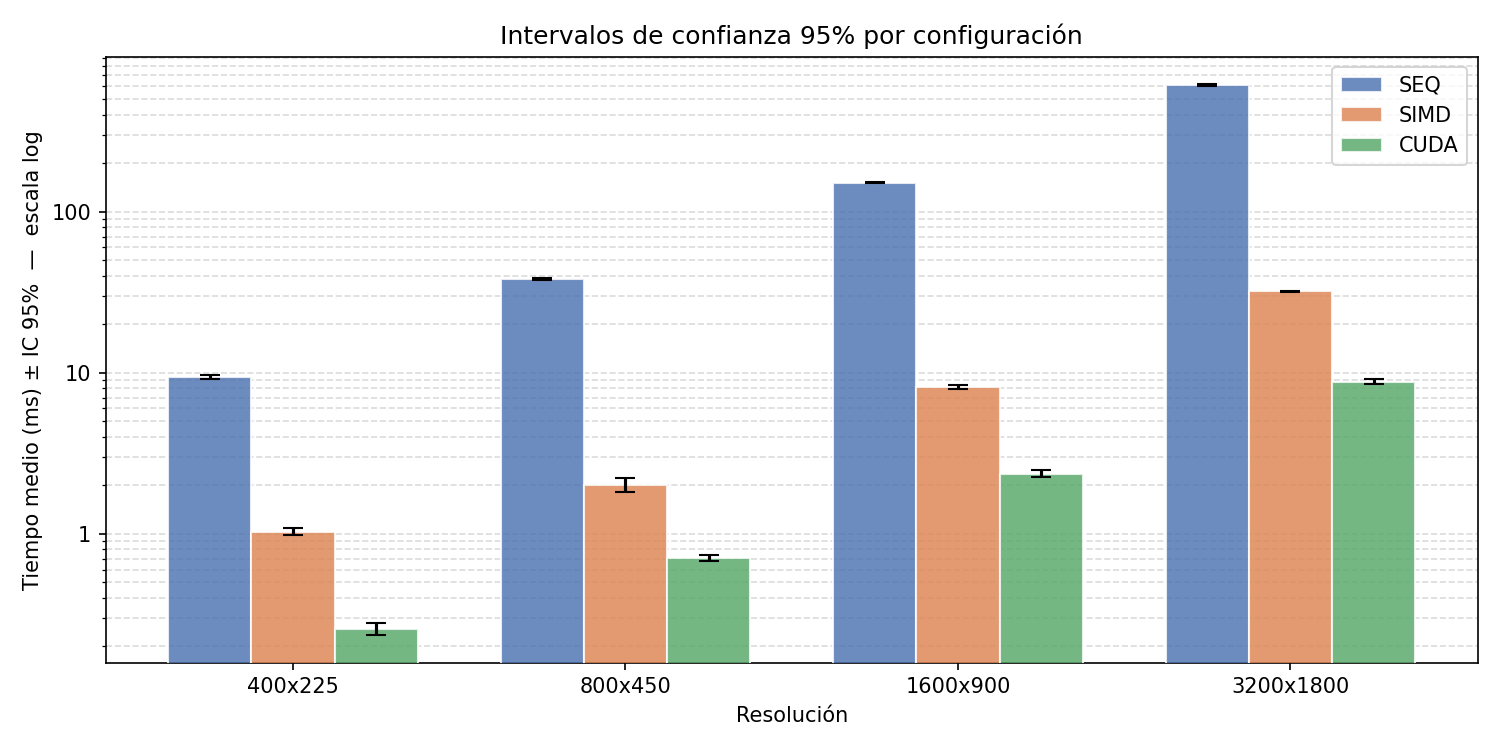
\includegraphics[width=\linewidth]{graficas/intervalos_confianza.png}
    \caption{Intervalos de confianza al 95\,\%.}
  \end{subfigure}
  \caption{Variabilidad estadística de las mediciones.}
  \label{fig:variab}
\end{figure}

% ---------------------------------------------------------------
\section{Variables Más Significativas para Aumentar la Paralelización}

A continuación se identifican las variables del algoritmo de ray tracing que tienen
el mayor impacto sobre el grado de paralelismo explotable.

\subsection{Variables de Primer Orden}

\begin{enumerate}

  \item \textbf{Ancho del tile / bloque de procesamiento ($W_t \times H_t$)}.
    En SIMD determina cuántos píxeles se empaquetan por iteración (actualmente 8).
    En CUDA determina la ocupación del SM (actualmente $16\!\times\!16 = 256$ hilos/bloque).
    Aumentar el ancho del tile en SIMD a 16 (AVX-512) o usar bloques de $32\!\times\!8$
    en CUDA puede mejorar la utilización del hardware.

  \item \textbf{Número de muestras por píxel (anti-aliasing, $N_{spp}$)}.
    Con $N_{spp} > 1$ cada píxel genera múltiples rayos independientes, incrementando
    linealmente el paralelismo disponible sin aumentar las dependencias de datos.

  \item \textbf{Profundidad máxima de reflexión ($D_{max}$)}.
    En la versión completa, cada rebote genera un rayo independiente. Explotar este
    paralelismo requiere un stack de rayos por hilo o una cola de trabajo (\textit{wavefront rendering}).

  \item \textbf{Número de primitivas de la escena ($N_s$)}.
    Con una BVH (\textit{Bounding Volume Hierarchy}), las $N_s$ intersecciones dejan de
    ser un bucle secuencial por rayo y se convierten en un recorrido paralelo del árbol,
    reduciendo la complejidad de $O(N_s)$ a $O(\log N_s)$ por hilo.

  \item \textbf{Coeficiente de reflectividad ($\rho$)}.
    Materiales con $\rho > 0$ generan rayos secundarios. Si $\rho = 0$ para la mayoría
    de primitivas, los hilos terminan antes y hay divergencia de warp. Minimizar la
    divergencia balanceando materiales mejora la eficiencia.

\end{enumerate}

\subsection{Variables de Segundo Orden}

\begin{enumerate}

  \item \textbf{Layout de memoria del framebuffer} (AoS vs.\ SoA).
    El diseño SoA actual en CUDA (tres arreglos separados \texttt{fb\_r}, \texttt{fb\_g},
    \texttt{fb\_b}) garantiza accesos coalescentes. Revertirlo a AoS degradaría el
    ancho de banda efectivo de escritura hasta en $3\!\times$.

  \item \textbf{Tipo de dato flotante} (\texttt{float32} vs.\ \texttt{float16}).
    Usar \texttt{half} en la GPU permite duplicar el ancho de banda de memoria y
    aprovechar las Tensor Cores en operaciones matriciales (útil para denoising).

  \item \textbf{Ancho de warp / lane width} (32 hilos en CUDA, 8 floats en AVX2).
    Variables que no alinean su dominio a este ancho generan hilos inactivos en el
    borde de la imagen. Padding de la resolución a múltiplos de 32 (CUDA) u 8 (SIMD)
    elimina este desperdicio.

  \item \textbf{Intensidad aritmética por rayo}.
    Agregar iluminación Phong y rayos de sombra incrementa la razón
    FLOP/byte, haciendo el kernel \textit{compute-bound} en lugar de
    \textit{memory-bound}, lo que beneficia la GPU.

\end{enumerate}

% ---------------------------------------------------------------
\section{Esquema DLP de las Partes del Problema}

El principio DLP (\textit{Data-Level Parallelism}) se manifiesta en diferentes
sub-etapas del ray tracing. La Figura~\ref{fig:dlp_schema} muestra el esquema completo.

\begin{figure}[H]
\centering
\resizebox{\linewidth}{!}{%
\begin{tikzpicture}[
  mainblock/.style={rectangle, draw=black, fill=gray!10,
                    minimum width=3.2cm, minimum height=0.8cm,
                    align=center, font=\small\bfseries},
  dlpblock/.style={rectangle, draw=rayblue, fill=rayblue!15,
                   minimum width=3.2cm, minimum height=0.7cm,
                   align=center, font=\scriptsize},
  simdlabel/.style={rectangle, draw=simdgreen, fill=simdgreen!15,
                    minimum width=2.8cm, minimum height=0.55cm,
                    align=center, font=\scriptsize},
  cudalabel/.style={rectangle, draw=gpuorange, fill=gpuorange!15,
                    minimum width=2.8cm, minimum height=0.55cm,
                    align=center, font=\scriptsize},
  arrow/.style={-{Stealth}, thick},
  dlparrow/.style={-{Stealth}, thick, rayblue!70}
]

% Columna 1 — sub-problemas
\node[mainblock] (cam)  at (0, 0)    {Generación\\de rayos};
\node[mainblock] (inter)at (0,-1.4)  {Intersección\\rayo-esfera};
\node[mainblock] (shade)at (0,-2.8)  {Shading\\Phong};
\node[mainblock] (shadow)at(0,-4.2)  {Rayos de\\sombra};
\node[mainblock] (refl) at (0,-5.6)  {Reflexión\\recursiva};
\node[mainblock] (store)at (0,-7.0)  {Escritura\\framebuffer};

\draw[arrow] (cam)   -- (inter);
\draw[arrow] (inter) -- (shade);
\draw[arrow] (shade) -- (shadow);
\draw[arrow] (shadow)-- (refl);
\draw[arrow] (refl)  -- (store);

% Columna 2 — tipo de DLP
\node[dlpblock] (dlp_cam)   at (4.2, 0)    {DLP: 1 rayo/píxel\\N×M píxeles independientes};
\node[dlpblock] (dlp_inter) at (4.2,-1.4)  {DLP: cálculo $b^2\!-\!ac$\\idéntico por rayo};
\node[dlpblock] (dlp_shade) at (4.2,-2.8)  {DLP: Phong por píxel\\sin dependencias cruzadas};
\node[dlpblock] (dlp_shadow)at (4.2,-4.2)  {DLP: rayo de sombra\\independiente por luz};
\node[dlpblock] (dlp_refl)  at (4.2,-5.6)  {DLP limitado: dependencia\\de profundidad (wavefront)};
\node[dlpblock] (dlp_store) at (4.2,-7.0)  {DLP: escritura independiente\\a posición única};

% Columna 3 — implementación
\node[simdlabel] (s_cam)    at (8.2, 0.25)  {SIMD: 8 rayos/iter.\\CUDA: 1 hilo/píxel};
\node[simdlabel] (s_inter)  at (8.2,-1.15)  {SIMD: FMA\_ps ×8\\CUDA: kernel escalar};
\node[simdlabel] (s_shade)  at (8.2,-2.55)  {SIMD: blend ×8\\CUDA: 1 hilo/píxel};
\node[cudalabel] (s_shadow) at (8.2,-4.45)  {CUDA: 1 hilo/rayo\\sombra (futuro)};
\node[cudalabel] (s_refl)   at (8.2,-5.85)  {CUDA: wavefront BFS\\(futuro Demo 3)};
\node[simdlabel] (s_store)  at (8.2,-6.75)  {SIMD: store\_ps\\CUDA: SoA coalescente};

% Flechas de conexión
\foreach \src/\dst in {cam/dlp_cam, inter/dlp_inter, shade/dlp_shade,
                        shadow/dlp_shadow, refl/dlp_refl, store/dlp_store}{
  \draw[dlparrow] (\src) -- (\dst);
}

% Etiquetas de columnas
\node[font=\small\bfseries] at (0, 0.85)   {Sub-problema};
\node[font=\small\bfseries, text=rayblue] at (4.2, 0.85) {Tipo de DLP};
\node[font=\small\bfseries, text=simdgreen!60!gpuorange] at (8.2, 0.85) {Implementación};

\end{tikzpicture}
}
\caption{Esquema DLP completo del ray tracer: sub-problemas, naturaleza del paralelismo
         de datos y mapeo a las implementaciones SIMD y CUDA.}
\label{fig:dlp_schema}
\end{figure}

% ---
\subsection{Análisis por Sub-problema}

\begin{description}
  \item Generación de rayos: Paralelismo perfecto: la dirección del rayo para el píxel
    $(x,y)$ depende únicamente de las coordenadas normalizadas $(u,v)$ y de los
    parámetros fijos de la cámara. No existe dependencia entre píxeles.

  \item Intersección rayo-esfera: El cálculo del discriminante
    $\Delta = (\mathbf{d}\cdot\mathbf{b})^2 - \|\mathbf{d}\|^2(
      \|\mathbf{b}\|^2 - r^2)$
    aplica las mismas operaciones a datos distintos (dirección del rayo), alineándose
    directamente con el modelo SIMD. Con $N_s = 5$ esferas el bucle es corto y
    completamente vectorizable.

  \item Shading Phong: Tres evaluaciones independientes (ambiental, difusa, especular)
    por píxel. La componente difusa requiere $\mathbf{N}\cdot\mathbf{L}$, que es un
    producto punto vectorizable. El DLP es total entre píxeles distintos.

  \item Rayos de sombra: Cada fuente de luz genera un rayo de sombra independiente.
    Con dos fuentes y $1\,440\,000$ píxeles esto equivale a $2.88\!\times\!10^6$ tests
    independientes, todos paralelizables.

  \item Reflexión recursiva: Es el único sub-problema con dependencia de datos: el rayo
    de nivel $k$ depende del hit del nivel $k-1$. La estrategia \textit{wavefront rendering}
    (procesar todos los rayos del mismo nivel en paralelo) convierte la recursión en
    iteraciones DLP puras.

  \item Escritura al framebuffer: Cada hilo escribe en una posición única
    (\texttt{idx = py*W + px}), sin conflictos. Con layout SoA los accesos de un warp
    son completamente coalescentes.
\end{description}

% ---------------------------------------------------------------
\section{Trabajo Pendiente para Demo 3}

\begin{itemize}
  \item Implementar Phong + rayos de sombra en SIMD (vectorizar también el shading).
  \item Implementar Phong + rayos de sombra en CUDA (el kernel ya soporta la extensión).
  \item Explorar \textit{wavefront rendering} para reflexiones en GPU.
  \item Medir speedup real con la misma carga de trabajo en las tres implementaciones.
  \item Evaluar el impacto de BVH en la etapa de intersección ($O(N_s) \to O(\log N_s)$).
\end{itemize}

% ---------------------------------------------------------------
\begin{thebibliography}{9}
\bibitem{shirley}
  P.\ Shirley, \textit{Ray Tracing in One Weekend}, 2020.
  \url{https://raytracing.github.io}
\bibitem{intel_avx}
  Intel Corporation, \textit{Intel Intrinsics Guide}, 2024.
  \url{https://www.intel.com/content/www/us/en/docs/intrinsics-guide}
\bibitem{cuda_prog}
  NVIDIA Corporation, \textit{CUDA C++ Programming Guide}, v12.x, 2024.
  \url{https://docs.nvidia.com/cuda/cuda-c-programming-guide}
\bibitem{pharr}
  M.\ Pharr, W.\ Jakob, G.\ Humphreys, \textit{Physically Based Rendering}, 4th ed., 2023.
\end{thebibliography}

\end{document}
